\documentclass[11pt,letterpaper]{article}
\usepackage{fullpage}
\usepackage[top=1.5cm, bottom=4.5cm, left=2cm, right=2cm]{geometry}
\usepackage[utf8]{inputenc}
\usepackage[spanish]{babel}
\usepackage{fancyhdr}
\usepackage{enumitem}
\usepackage{float}
\usepackage{graphicx}

\spanishdecimal{.}

\setlength{\parindent}{0.0in}
\setlength{\parskip}{0.05in}

\newcommand\course{Modelación basada en agentes} % Materia
\newcommand\hwType{Práctica 2} % Tipo de tarea
\newcommand\StudentNameA{González Alvarado Raúl} % Nombre
\newcommand\StudentNameB{} % Nombre

\pagestyle{fancyplain}
\headheight 35pt
\lhead{\StudentNameA\\\StudentNameB}
\rhead{\course \\ \today}
\chead{\textbf{\Large \hwType}}
\cfoot{}
\rfoot{\small\thepage}
\headsep 1cm

\begin{document}
    \section{Algoritmo genético simple}
    \begin{enumerate}[label=\alph*)]
        \item Escribe la modelación de las posibles soluciones:
        
        Se usó una cadena de binarios que representa el genotipo, la longitud de la cadena es de 18 dígitos ya que con la conversión utilizada (binario a flotante entre 0 y 1) se necesita de un decimal de 9 dígitos para que nuestro fenotipo pueda tener una presición de 6 decimales y al necesitar una coordenada $x$ y una $y$ se necesita $2*9$ bits. El proceso usado para convertir de genotipo a fenotipo es el siguiente:
        \begin{enumerate}[label=\arabic*.]
            \item Dividir la lista binaria en partes iguales.
            \item Pasar cada lista binaria $[b_1, ..., b_9]$ a la función \texttt{bit\_string\_to\_float} $= \sum_{i \in 1...9} b_i * 10^{-i}$
            \item Normalizar el valor regresado en el paso anterior a la función \texttt{normaliza\_fenotipo}, que convierte el número flotante en un número entre el rango $[-500, 500]$
        \end{enumerate}

        \item Establecer una población fija de 100 individuos, la tasa de recombinación en $P_c =0.5$, la tasa de mutación en $P_m=0.1$, la condición de término en 500 generaciones. ¿Cuál fue el mejor individuo al terminar la ejecución? Reporte la estructura del genotipo, fenotipo y fitness ¿es el máximo global?
        
        El mejor individuo generado en una ejecución aleatoria fue:
        \begin{enumerate}
            \item Genotipo:  $[1, 1, 1, 0, 1, 0, 1, 0, 1, 1, 1, 1, 0, 1, 1, 1, 0, 1]$
            \item Fenotipo:  $[416.015625, 431.640625]$
            \item Schwefel(Fenotipo):  820.5315588989117
        \end{enumerate}
        
        No es el máximo global pero está muy cerca. Las gráfica obtenidas fueron:
        
        \begin{enumerate}[label=\arabic*.]
            \item Generación vs Fitness:
            \begin{figure}[H]
                \centering
                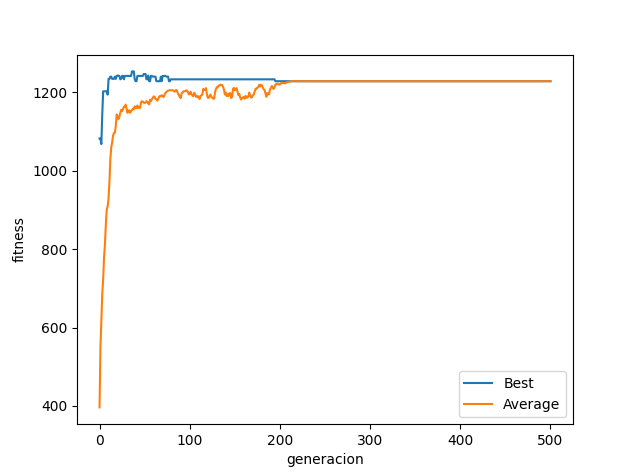
\includegraphics[width=8cm]{images/gen-vs-fitness.png}
                \label{fig:gen-vs-fit}
            \end{figure}
            
            \item Distintas generaciones:
            \begin{figure}[H]
                \centering
                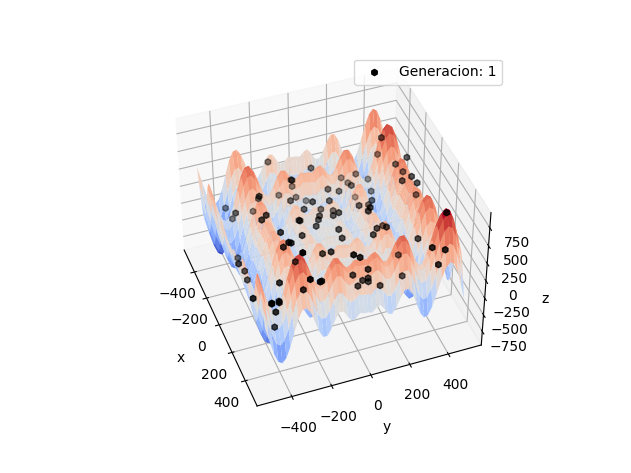
\includegraphics[width=8cm]{images/gen001.png}
                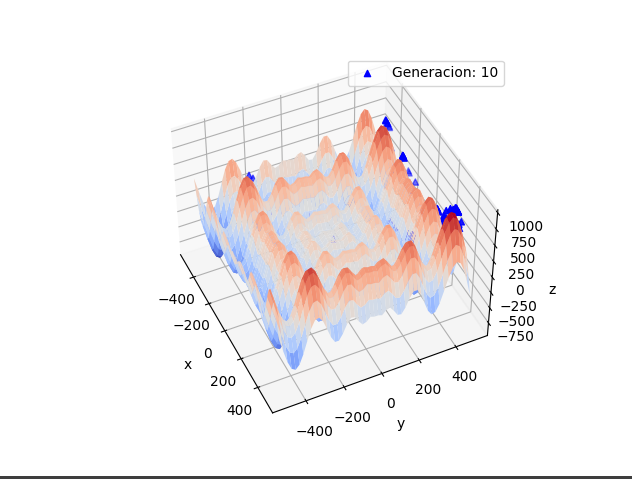
\includegraphics[width=8cm]{images/gen010.png}
                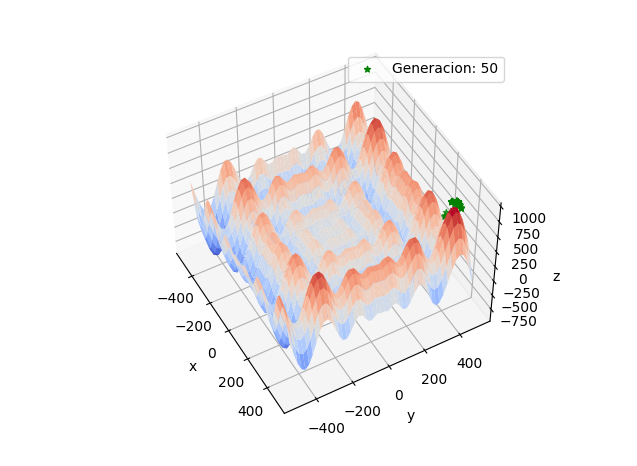
\includegraphics[width=8cm]{images/gen050.png}
                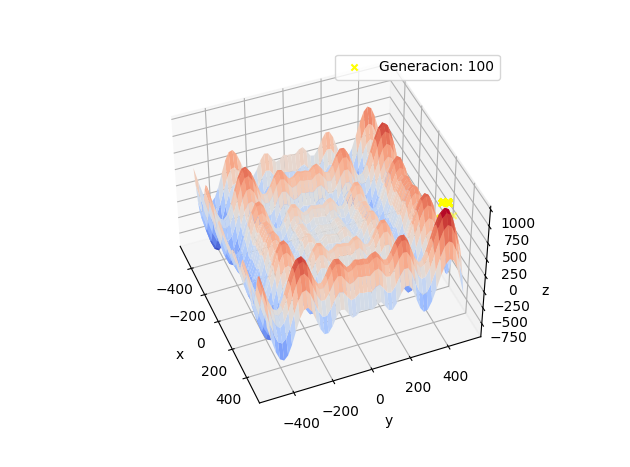
\includegraphics[width=8cm]{images/gen100.png}
                \label{fig:gen-n}
            \end{figure}
        \end{enumerate}

        \item Genere otros experimentos cambiando la tasa de recombinación y de mutación. A partir de su experiencia trate de ajustar los parámetros para que el AGS tenga el mejor desempeño posible y graficar como en los puntos anteriores. ¿Cuáles fueron los parámetros con los que encontraron rápidamente el máximo global? Explique.
        
        \begin{enumerate}[label=\arabic*.]
            \item Generación vs Fitness:
            \begin{figure}[H]
                \centering
                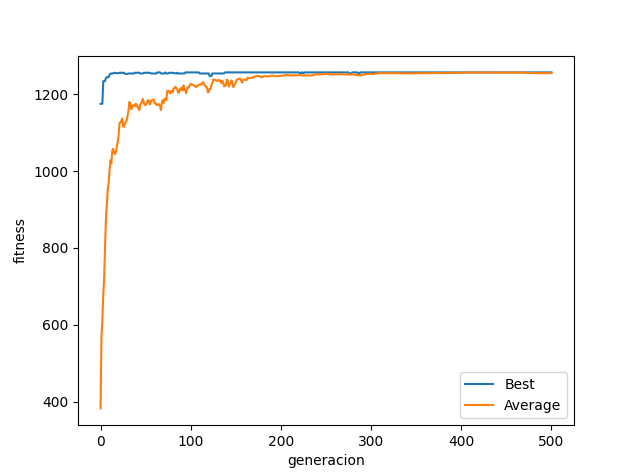
\includegraphics[width=8cm]{images/parametros-ajustados/parametros-gen-vs-fitness.png}
                \label{fig:parametros-gen-vs-fit}
            \end{figure}
            
            \item Distintas generaciones:
            \begin{figure}[H]
                \centering
                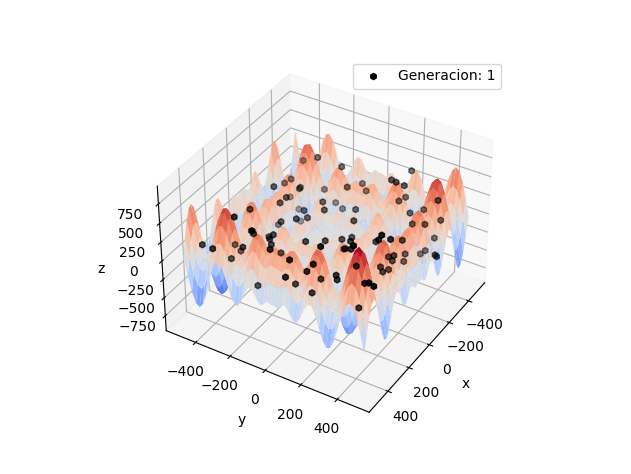
\includegraphics[width=8cm]{images/parametros-ajustados/parametros-gen001.png}
                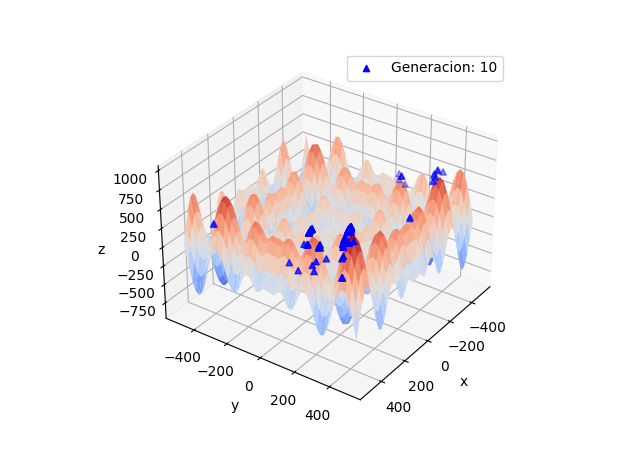
\includegraphics[width=8cm]{images/parametros-ajustados/parametros-gen010.png}
                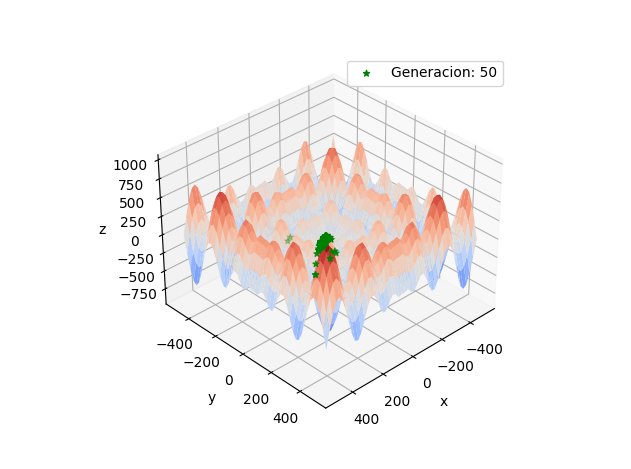
\includegraphics[width=8cm]{images/parametros-ajustados/parametros-gen050.png}
                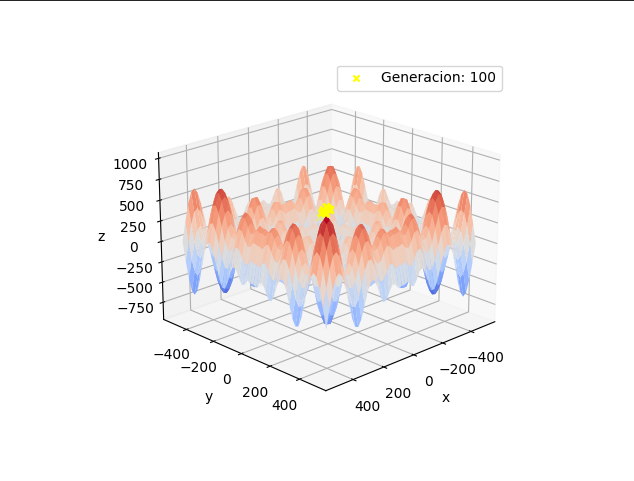
\includegraphics[width=8cm]{images/parametros-ajustados/parametros-gen100.png}
                \label{fig:parametros-gen-n}
            \end{figure}
        \end{enumerate}
        
        Se usaron los parámetros siguientes: $P_c = 0.5$ y $P_m = 0.01$. La taza de mutación se mantuvo en 0.5, ya que al ser el tamaño de la población relativamente grande se alcanzaba a generar muy buenos individuos casi desde las primeras generaciones. Para mantener estos individuos a lo largo de las generaciones solamente se hizo la cruza entre la mitad de los individuos seleccionados. Para la mutación se mantuvo lo más baja posible para que solamente en caso de que al inicio no tengamos individuos buenos puedan cambiar y adaptarse hasta obtener uno relativamente bueno.
    \end{enumerate}
\end{document}